\documentclass[11pt]{article}
\usepackage{geometry}
\geometry{letterpaper, margin=1in}
\usepackage[utf8]{inputenc}
\usepackage{graphicx}
\usepackage{upgreek}
\usepackage{hyperref}
\usepackage[T1]{fontenc}
\usepackage{amsmath}
\usepackage[colorinlistoftodos]{todonotes}
\usepackage{float}
\usepackage{minted} 

\title{ECE532S Digital Systems Design \\ \vspace{0.4cm}
       \Large Tutorial 7 - Simulating AXI Interfaces Using the AXI VIP \\ \vspace{0.4cm}
       \small Last Updated: July, 2020}
\author{ }
\date{ }

\begin{document}
\maketitle
\vspace{-1cm}

The goal of this tutorial is to demonstrate how to use the Xilinx AXI Verification IP (VIP) to test and verify an AXI lite peripheral using the Xilinx Vivado Simulator. This tutorial will demonstrate how to connect the VIP to your design and use it to write to and read from registers of an AXI lite IP Core, in particular the AXI GPIO core.

\section{Create Project with an AXI VIP}
\label{sec:create_proj}
\begin{enumerate}
    \item Create a new project, with no sources or constraints for now, targeting the FPGA on the \textit{Nexsys} board (\textbf{xc7a100tcsg324-1}), as has been demonstrated in previous tutorials. 
    \item Create a new block design and name it \textbf{design\_1}. In the block diagram, add an \textit{AXI Verification IP} (the AXI VIP) and an \textit{AXI GPIO} Core. 
    \item \textbf{Double click} the VIP Core to bring up the configuration window and ensure the \textit{INTERFACE MODE} is set to \textbf{MASTER} (see Figure~\ref{fig:axivipconfig}). This will set the AXI VIP into master mode, such that it can initiate reads and writes. Note, the \textit{PROTOCOL} field is set to auto, as Vivado can deduce from the port it is connected to which protocol to use. 
    
    \begin{figure}[H]
      \centering
      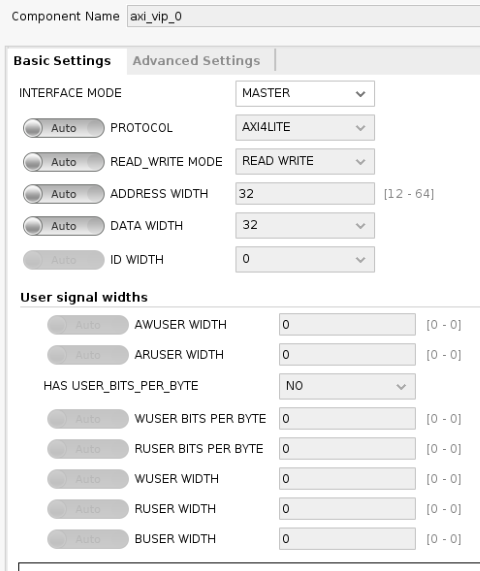
\includegraphics[width=0.5\textwidth]{axivipconfig.png}
      \caption{AXI VIP configuration window, basic settings}
      \label{fig:axivipconfig}
    \end{figure}
    
    \item Next, we need to configure the AXI GPIO Core. \textbf{Double click} the GPIO Core to bring up the configuration window. Set \textit{GPIO Width} under \textit{GPIO} to \textbf{16}, and place a checkmark by \textit{Enable Dual Channel}. This will allow us to enable and modify the settings of GPIO2. Place a checkmark by \textit{All inputs}, and set \textit{GPIO Width} under \textit{GPIO2} to \textbf{5}. Your settings should look like the settings in Figure \ref{fig:gpiocoresettings}. Press \textbf{OK} to save.
    
    \begin{figure}[H]
      \centering
      \includegraphics[width=0.6\textwidth]{gpio_core_settings.png}
      \caption{GPIO Core configuration window, basic settings}
      \label{fig:gpiocoresettings}
    \end{figure}
    
    \item Connect the \textit{M\_AXI} signal of the VIP to the \textit{S\_AXI} signal of the GPIO, an AXI lite protocol signal. If you find that the signals will not connect, re-open the VIP Core's configuration window and verify that \textit{PROTOCOL} is set to \textbf{AXI4LITE} (manually change the setting if necessary).
    
    \item Add and wire the \textbf{AXI Verification IP}, \textbf{AXI GPIO}, and \textbf{Constant} IPs to the diagram as shown in Figure \ref{fig:bd} below. Make sure that the port names match the figure. The \textbf{aclk} port should be set as an \textbf{Input} \textbf{Clock} port with frequency \textbf{100MHz}. The \textbf{aresetn} port should be set as an \textbf{Input} \textbf{Reset} port set to \textbf{Active Low}. The \textit{leds} port should be set as an \textbf{Output} \textbf{Other} port which is a \textbf{vector} from \textbf{15 to 0}.
    
    \begin{figure}[H]
      \centering
      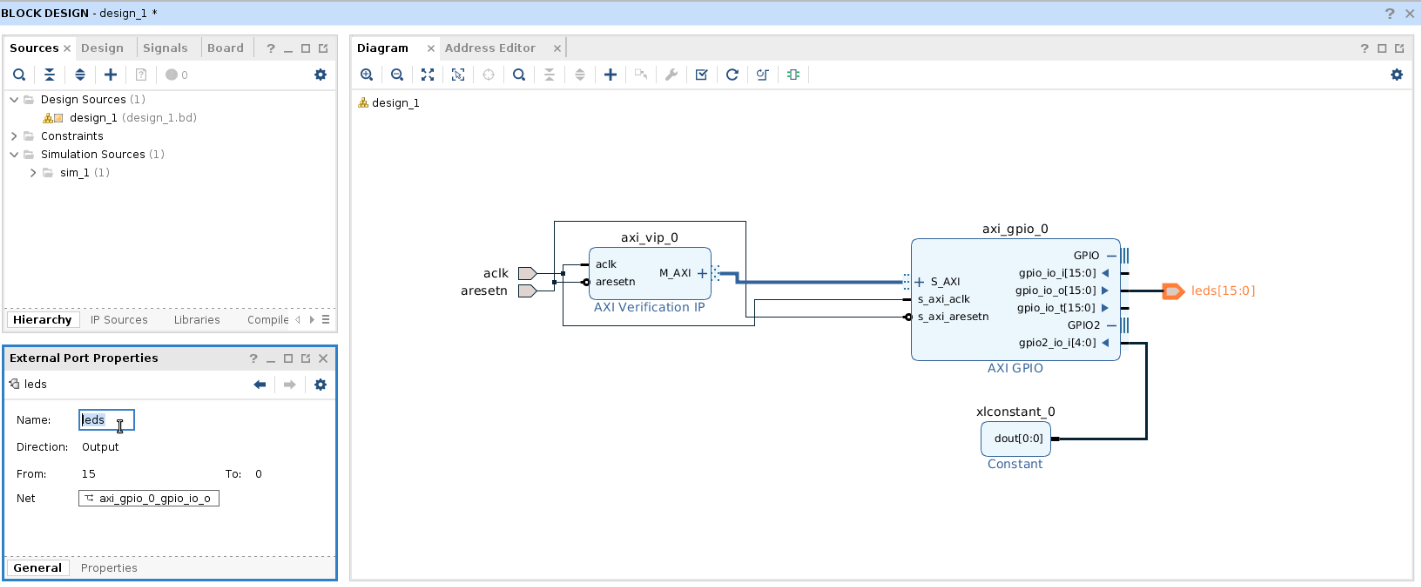
\includegraphics[width=\textwidth]{bd.png}
      \caption{Block design.}
      \label{fig:bd}
    \end{figure}

    % \item Configure the \textbf{AXI GPIO IP} as shown in the following figure. We will be using the VIP to set the LEDs and read from the push buttons.
    
    % \begin{figure}[H]
    %   \centering
    %   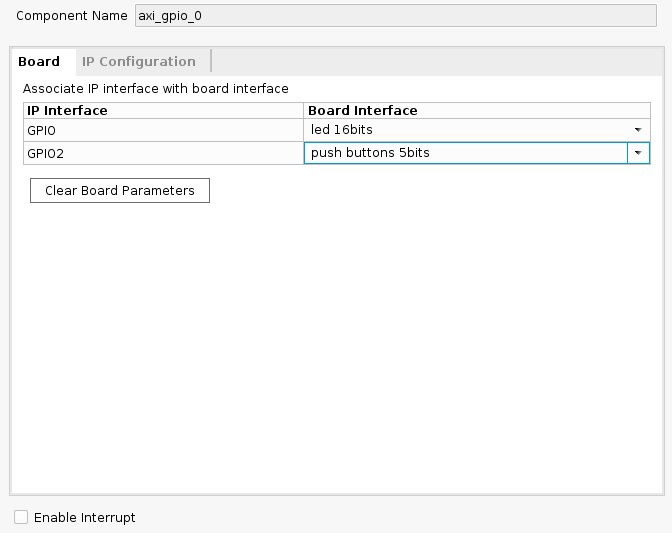
\includegraphics[scale=0.5]{axigpioconfig.png}
    %   \caption{AXI GPIO configuration window.}
    %   \label{fig:axigpioconfig}
    % \end{figure}
    
    \item Configure the \textbf{Constant} IP as shown in Figure \ref{fig:axiconstantconfig}. The constant value of 5 will simulate pushing buttons 0 and 2.
    
    \begin{figure}[H]
      \centering
      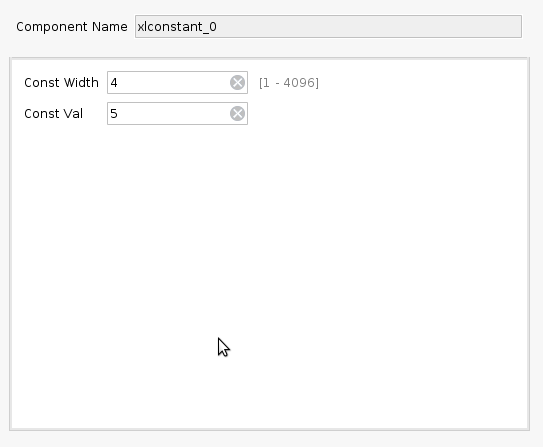
\includegraphics[scale=0.5]{axiconstantconfig.png}
      \caption{Constant configuration window.}
      \label{fig:axiconstantconfig}
    \end{figure}
    
    \item Go the \textbf{address editor} tab and set the offset address to \textbf{0x40000000} (see Figure \ref{fig:addresseditor}). If the GPIO Core (\textit{axi\_gpio\_0}) is \textit{unmapped}, click and drag the entire row into \textbf{MASTER\_AXI} to map it.
    
    \begin{figure}[H]
      \centering
      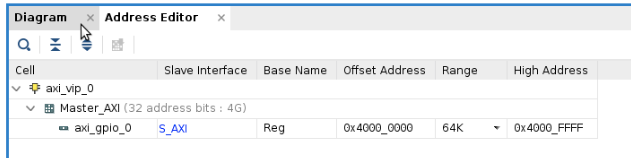
\includegraphics[scale=0.5]{addresseditor.png}
      \caption{Address Editor}
      \label{fig:addresseditor}
    \end{figure}
    
    \item Validate the block design, create the HDL wrapper, and generate the block design. 
    
    \begin{figure}[H]
      \centering
      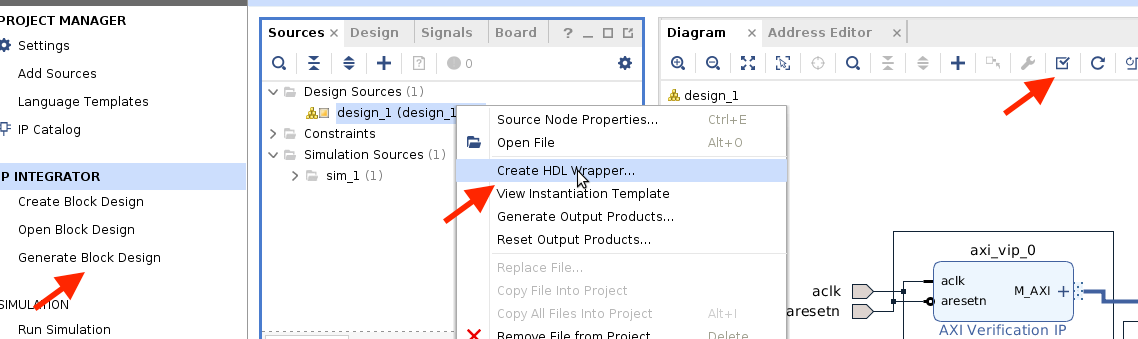
\includegraphics[scale=0.4]{validatebd.png}
      \caption{Generating the block design files.}
      \label{fig:validatebd.png}
    \end{figure}
\end{enumerate}

\newpage
\section*{Step 2: Creating the testbench}
\begin{enumerate}
	\item Import \textbf{tb.sv} as a \textbf{simulation source}. 	
		\begin{figure}[H]
		  \centering
		  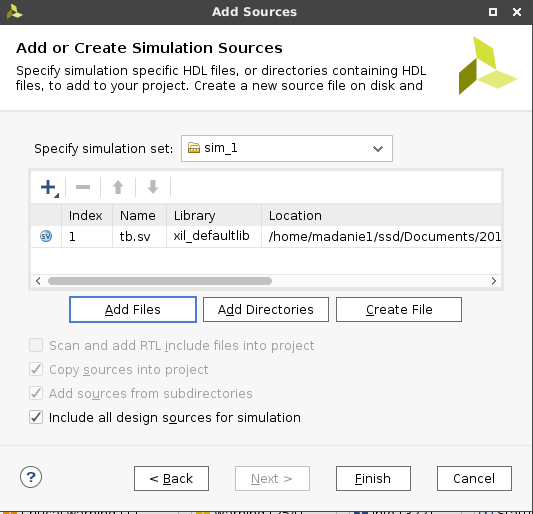
\includegraphics[scale=0.4]{addsimfiles.png}
		  \caption{Importing testbench files.}
		  \label{fig:addsimfilespng}
		\end{figure}
	\item Open the tb.sv file in Vivado text editor. Replace the \textbf{\textless vip\_component\_name\textgreater} in line 4 and 15 with the vip component name. Refer to Figure \ref{fig:findnames} to determine what the component name is for your design.
		\begin{figure}[H]
		  \centering
		  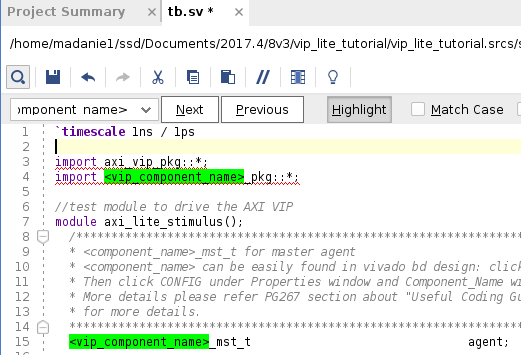
\includegraphics[scale=0.5]{componentname1.png}
		  \caption{Replace lines 4 and 15 with the appropriate component name for your VIP.}
		  \label{fig:componentname1}
		\end{figure}
		\begin{figure}[H]
		  \centering
		  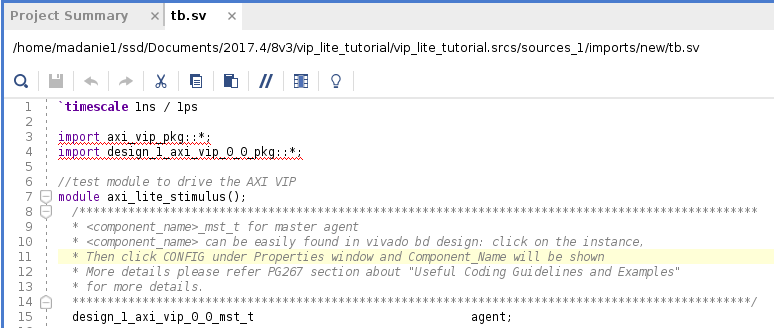
\includegraphics[scale=0.5]{componentname2.png}
		  \caption{Example of what lines 4 and 15 should look like.}
		  \label{fig:componentname2}
		\end{figure}
		\begin{figure}[H]
		  \centering
		  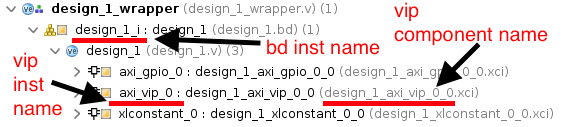
\includegraphics[scale=0.5]{filehierarchy2.png}
		  \caption{How to find the component and instance name.}
		  \label{fig:findnames}
		\end{figure}
		
	\item Go to line 60, and replace \textbf{\textless bd\_instance\_name\textgreater} and \textbf{\textless vip\_instance\_name\textgreater} with the bd instance name and vip instance name. Refer to Figure \ref{fig:findnames} to determine what the instance names are for your design.
		\begin{figure}[H]
		  \centering
		  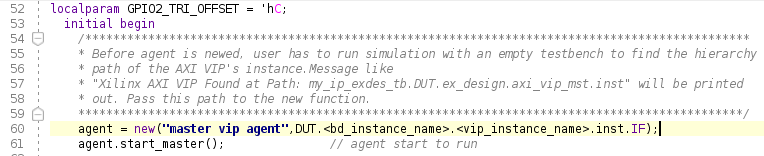
\includegraphics[scale=0.5]{instancename1.png}
		  \caption{Replace line 60 with the appropriate instance names for your BD and VIP.}
		  \label{fig:instancename1}
		\end{figure}
				\begin{figure}[H]
		  \centering
		  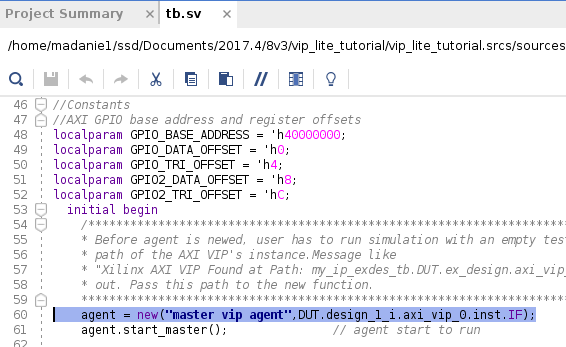
\includegraphics[scale=0.5]{instancename2.png}
		  \caption{Example of what line 60 should look like.}
		  \label{fig:instancename2}
		\end{figure}
	\item Set tb instance under Simulation Sources as the top instance if it isn't already. The simulation source hierarchy should look like the figure below. 
		\begin{figure}[H]
		  \centering
		  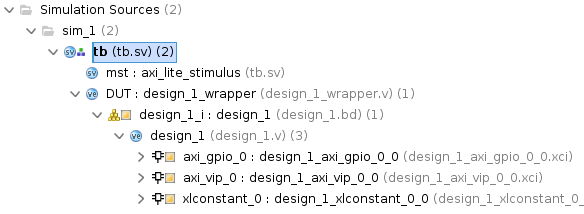
\includegraphics[scale=0.5]{filehierarchy.png}
		  \caption{Simulation source hierarchy.}
		  \label{fig:filehierarchy}
		\end{figure} 
\end{enumerate}
\section*{Step 3: Simulate the testbench}
\begin{enumerate}
	\item Before simulation, go to tb.sv and analyze line 66 to 75. This is where our test vectors are located. We will be writing to the output register of the GPIO bank that is connected to the LEDs. Then we'll set the push button GPIOs to be inputs and then wait for all writes to finish. We will then read the GPIO data register for the push buttons, and print the value of that register to the tcl console.
		\begin{figure}[H]
		  \centering
		  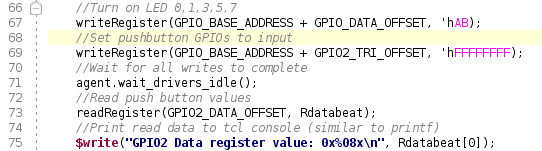
\includegraphics[scale=0.5]{tbanalysis.png}
		  \caption{TB test vectors.}
		  \label{fig:tbanalysis}
		\end{figure} 
	\item  Start the simulation by clicking \textbf{Run Simulation $\rightarrow$ Run Behavioural Simulation} on the navigation pane. Add the AXI bus signals in the \textit{Objects} window (Make sure that you select the VIP instance in the \textit{Scope} window) to the simulation window, shown in Figure \ref{fig:addtbsignals}. Relaunch the simulation by clicking the \textbf{Relaunch} button shown in Figure \ref{fig:relaunch}.
		\begin{figure}[H]
		  \centering
		  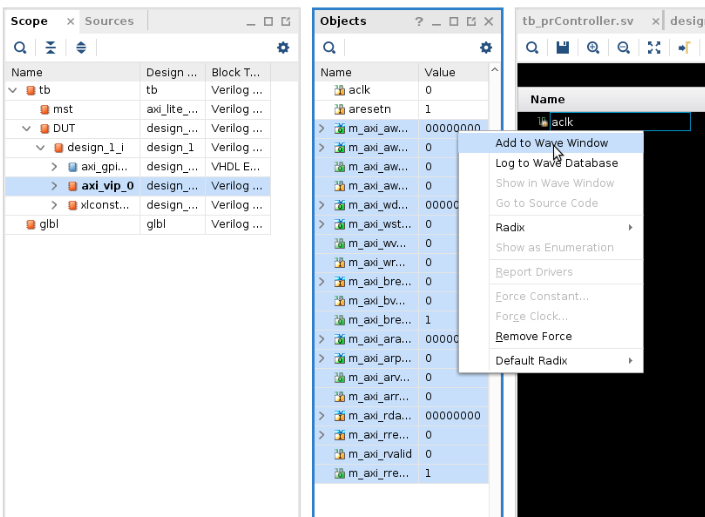
\includegraphics[scale=0.5]{addtbsignals.png}
		  \caption{Adding AXI signals to the simulation.}
		  \label{fig:addtbsignals}
		\end{figure} 
		\begin{figure}[H]
		  \centering
		  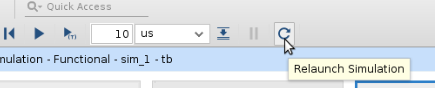
\includegraphics[scale=0.5]{relaunch.png}
		  \caption{Relaunching the simulation.}
		  \label{fig:relaunch}
		\end{figure} 
	\item Analyze the tb results. The waveform should look like Figure \ref{fig:simwaveform.png}. In the \textit{Tcl Console} you should see \textit{GPIO2} returning \textit{0x00000005}, as seen in Figure \ref{fig:simruntclconsole}.
		\begin{figure}[H]
		  \centering
		  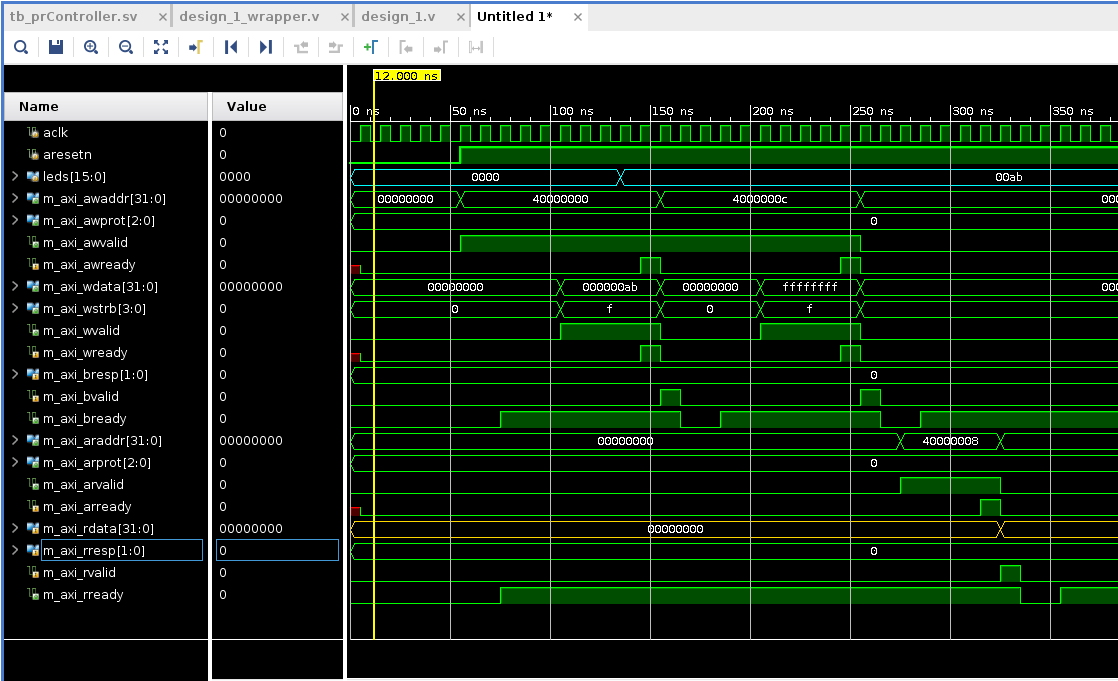
\includegraphics[scale=0.4]{simwaveform.png}
		  \caption{Simulation waveform.}
		  \label{fig:simwaveform.png}
		\end{figure} 
		\begin{figure}[H]
		  \centering
		  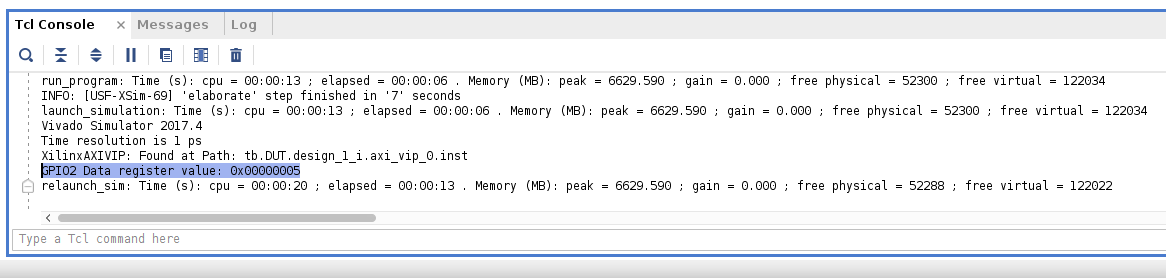
\includegraphics[scale=0.5]{simruntclconsole.png}
		  \caption{Tcl console print out of register.}
		  \label{fig:simruntclconsole}
		\end{figure} 
\end{enumerate}
\section*{Troubleshooting}
\begin{enumerate}
\item If the Vivado simulator bugs out and starts throwing errors that are not related to your source files, you can try to fix it by reseting your behaviour simulation.
		\begin{figure}[H]
		  \centering
		  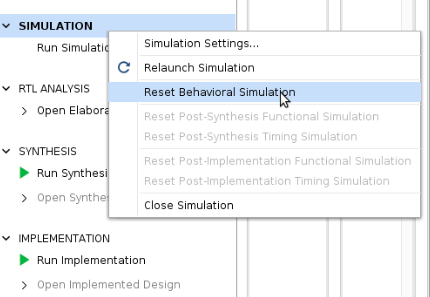
\includegraphics[scale=0.5]{troubleshoot1.png}
		  \caption{Resetting the simulation.}
		  \label{fig:roubleshoot1}
		\end{figure} 
\item If you want to create more advanced AXI testbenches with the Vivado AXI VIP refer to their example design.
		\begin{figure}[H]
		  \centering
		  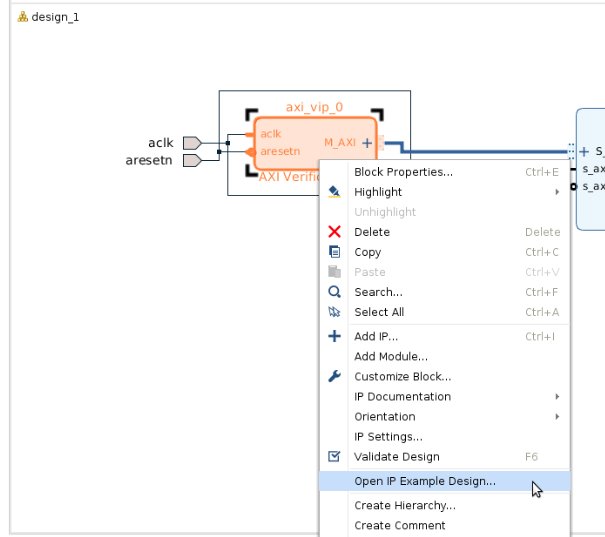
\includegraphics[scale=0.5]{exdesign.png}
		  \caption{Advanced example design for the AXI VIP.}
		  \label{fig:exdesign}
		\end{figure} 
\end{enumerate}


\end{document}
